%%%%%%%%%%%%%%%%%%%%%%%%%%%%%%%%%%%%%%%%%
% Ay 190 - WS2
% Written by Chatarin Wong-u-railertkun
%%%%%%%%%%%%%%%%%%%%%%%%%%%%%%%%%%%%%%%%%

%----------------------------------------------------------------------------------------
%	PACKAGES AND OTHER DOCUMENT CONFIGURATIONS
%----------------------------------------------------------------------------------------

\documentclass[11pt,letterpaper]{article}

% Load some basic packages that are useful to have
% and that should be part of any LaTeX installation.
%

\usepackage{graphicx}     % be able to include figures

\usepackage{xcolor}         % get nice colors

% change default font to Palatino (looks nicer!)
\usepackage[latin1]{inputenc}
\usepackage{mathpazo}
\usepackage[T1]{fontenc}

% load some useful math symbols/fonts
\usepackage{latexsym,amsfonts,amsmath,amssymb}
\usepackage{subcaption}

% comfort package to easily set margins
\usepackage[top=1in, bottom=1in, left=1in, right=1in]{geometry}

% control some spacings
%
% spacing after a paragraph
\setlength{\parskip}{.15cm}
% indentation at the top of a new paragraph
\setlength{\parindent}{0.0cm}

\usepackage{courier}


%----------------------------------------------------------------------------------------
%	TITLE
%----------------------------------------------------------------------------------------

\begin{document}

\begin{center}
\Large
Ay190 -- Worksheet 13 - N-body simulation \\    %%%%%% DON'T FORGET TO CHANGE THE WORK SHEET NUMBER
Chatarin (Mee) Wong-u-railertkun\\
Date: \today
\end{center}

\section{Earth-Sun system}

Using RK4 to perform the integration by Newtonian force for acceleration. If you run the code \texttt{Q2.py}, you can see the 3D simulation of the Earth-Sun system. Also, several information are also printed, including the iteration, time, and distance between the Earth and Sun. Initially, the distance is at 1.49599e+13 cm. But the distance is not exactly constant. The distance increases until it reaches the maximum at 1.49676e+13 cm, when the time is at half the period. Then the distance decreases back to the initial distance when the Earth completes the full cycle.

\section{Energy of Earth-Sun system}

As time progresses, the total energy is not really preserved. The total energy decreases. Figure ~\ref{fig:Energy_Cov} shows the convergence of the change in total energy with the resolution.

\begin{figure}[h!]
	\centering
	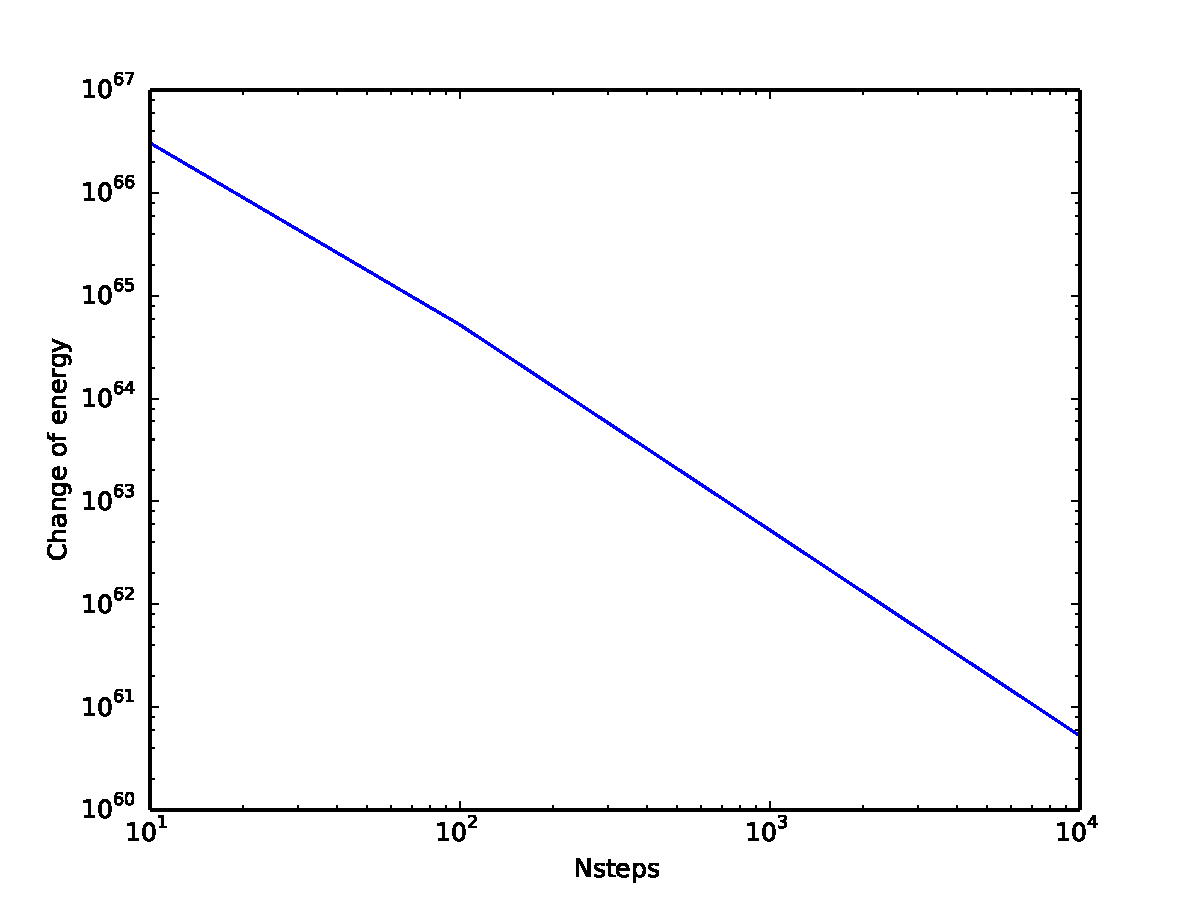
\includegraphics[width=0.5\textwidth]{Energy_Conv}
	\caption{}
	\label{fig:Energy_Cov}
\end{figure}

\section{Groups of star}
Figure \ref{fig:DeltaE} shows the change of the energy, i.e. initial energy minus the energy at the time, vs. time. We can see that the energy is not preserved, but the energy changes with a pattern and periodicity.


\begin{figure}[h!]
	\centering
	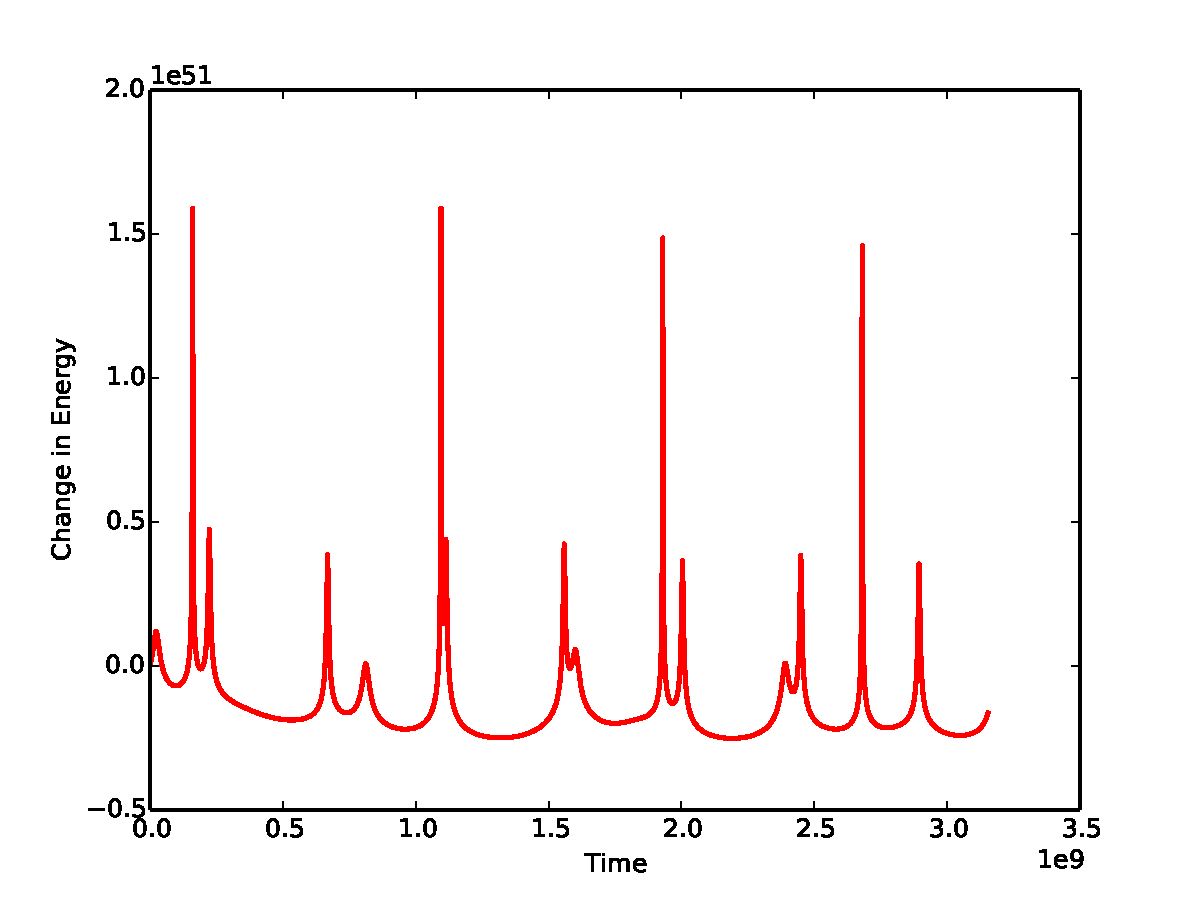
\includegraphics[width=0.5\textwidth]{DeltaE}
	\caption{}
	\label{fig:DeltaE}
\end{figure}
	
\end{document}

